\uuid{D5EP}
\exo7id{5908}
\titre{exo7 5908}
\auteur{rouget}
\organisation{exo7}
\datecreate{2010-10-16}
\isIndication{false}
\isCorrection{true}
\chapitre{Intégration}
\sousChapitre{Intégrale multiple}
\module{Analyse}
\niveau{L2}
\difficulte{}

\contenu{
\texte{
Calculer les intégrales multiples suivantes
}
\begin{enumerate}
    \item \question{$I=\displaystyle\iint_{D}(x+y)\;dxdy$ où $D=\{(x,y)\in\Rr^2/\;x\leqslant1,\;y\leqslant1,\;x+y\geqslant1\}$.}
\reponse{Représentons le domaine $D=\{(x,y)\in\Rr^2/\;x\leqslant1,\;y\leqslant1,\;x+y\geqslant1\}$.

$$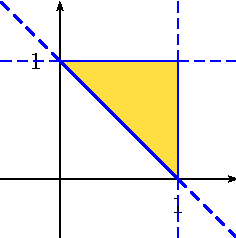
\includegraphics{../images/pdf/D5EP-1.pdf}$$



\begin{align*}\ensuremath
I&=\displaystyle\iint_{D}(x+y)\;dxdy=\int_{0}^{1}\left(\int_{1-x}^{1}(x+y)dy\right)dx\;(\text{ou aussi}\;\int_{0}^{1}\left(\int_{0}^{1-y}(x+y)dx\right)dy)\\
 &=\int_{0}^{1}\left[xy+ \frac{y^2}{2}\right]_{y=1-x}^{y=1}dx=\int_{0}^{1}\left(x+ \frac{1}{2}-x(1-x)- \frac{(1-x)^2}{2}\right)dx\\
 &=\int_{0}^{1}\left( \frac{x^2}{2}+x\right)dx= \frac{1}{6}+ \frac{1}{2}= \frac{2}{3}.
\end{align*}

\begin{center}
\shadowbox{
$\displaystyle\iint_{D}(x+y)\;dxdy= \frac{2}{3}$.
}
\end{center}}
    \item \question{$I=\displaystyle\iint_{[-1,1]^2}|x+y|\;dxdy$.}
\reponse{Si on pose pour $(x,y)\in/mbr^2$, $f(x,y)=|x+y|$ alors pour tout $(x,y)\in\Rr^2$, $f(-x,-y)=f(x,y)$ ou encore $f$ prend les mêmes valeurs en deux points symétriques par rapport à $O$. Puisque le point $O$ est centre de symétrie de $[-1,1]^2$, on en déduit que

\begin{align*}\ensuremath
I&=\displaystyle\iint_{-1\leqslant x,y\leqslant1,\;x+y\geqslant0}f(x,y)\;dxdy+\displaystyle\iint_{-1\leqslant x,y\leqslant1,\;x+y\leqslant0}f(x,y)\;dxdy\\
 &=2\iint_{-1\leqslant x,y\leqslant1,\;x+y\geqslant0}(x+y)\;dxdy=2\int_{-1}^{1}\left(\int_{-x}^{1}(x+y)\;dy\right)dx\\
 &=2\int_{-1}^{1}\left[xy+ \frac{y^2}{2}\right]_{y=-x}^{y=1}dx=2\int_{-1}^{1}\left(x+ \frac{1}{2}+x^2- \frac{x^2}{2}\right)dx\\
 &=2\left( \frac{1}{2}\times \frac{2}{3}+ \frac{1}{2}\times2\right)= \frac{8}{3}.
\end{align*}

\begin{center}
\shadowbox{
$\displaystyle\iint_{[-1,1]^2}|x+y|\;dxdy= \frac{8}{3}$.
}
\end{center}}
    \item \question{$I=\displaystyle\iint_{D}xy\;dxdy$ où $D$ est la partie du plan limitée par les paraboles d'équations respectives $y=x^2$ et $x=y^2$.}
\reponse{Représentons le domaine $D=\{(x,y)\in\Rr^2/\;0\leqslant x\leqslant1,\;0\leqslant y\leqslant1,\;x^2\leqslant y\leqslant\sqrt{x}\}$.

$$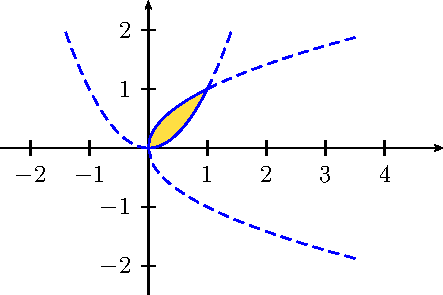
\includegraphics{../images/pdf/D5EP-2.pdf}$$


\begin{align*}\ensuremath
I&=\int_{0}^{1}\left(\int_{x^2}^{\sqrt{x}}y\;dy\right)x\;dx=\int_{0}^{1}x\left[ \frac{y^2}{2}\right]_{y=x^2}^{y=\sqrt{x}}\;dx= \frac{1}{2}\int_{0}^{1}x(x-x^4)\;dx= \frac{1}{2}\left( \frac{1}{3}- \frac{1}{6}\right)\\
&= \frac{1}{12}.
\end{align*}}
    \item \question{$I=\displaystyle\iint_{x^2+y^2\leqslant1} \frac{1}{1+x^2+y^2}\;dxdy$.}
\reponse{En passant en polaires, on obtient

\begin{align*}\ensuremath
I&=\iint_{x^2+y^2\leqslant1} \frac{1}{1+x^2+y^2}\;dxdy=\iint_{0\leqslant r\leqslant1,\;0\leqslant\theta\leqslant2\pi} \frac{1}{1+r^2}\;rdrd\theta\\
 &=\left(\int_{0}^{1} \frac{r}{1+r^2}\;dr\right)\times\left(\int_{0}^{2\pi}d\theta\right)\;(\text{intégrales indépendantes})\\
 &=2\pi\times\left[ \frac{1}{2}\ln(1+r^2)\right]_0^1=\pi\ln2.
\end{align*}

\begin{center}
\shadowbox{
$\displaystyle\iint_{x^2+y^2\leqslant1} \frac{1}{1+x^2+y^2}\;dxdy=\pi\ln2$.
}
\end{center}}
    \item \question{$I=\displaystyle\iint_{x\leqslant x^2+y^2\leqslant1} \frac{dxdy}{(1+x^2+y^2)^2}$.}
\reponse{Posons $D=\{(x,y)\in\Rr^2/\;x\leqslant x^2+y^2\leqslant1\}$. Puisque $x\leqslant x^2+y^2\Leftrightarrow\left(x- \frac{1}{2}\right)^2+y^2\geqslant \frac{1}{4}$, $D$ est l'intersection de l'intérieur du disque de centre $O$ et de rayon $1$, bord compris, et de l'extérieur du disque de centre $\left( \frac{1}{2},0\right)$ et de rayon $ \frac{1}{2}$, bord compris. Soit $M$ un point du plan. On note $(r,\theta)$ un couple de coordonnées polaires de $M$ tel que $r\geqslant0$ et $\theta\in[0,2\pi]$.

\begin{center}
$M\in D\Leftrightarrow r\cos\theta\leqslant r^2\leqslant1\Leftrightarrow r=0\;\text{ou}\;(0<r\leqslant1\;\text{et}\;r\geqslant\cos\theta$.
\end{center}

$$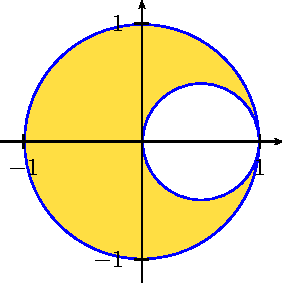
\includegraphics{../images/pdf/D5EP-3.pdf}$$


En passant en polaires, on obtient

\begin{align*}\ensuremath
I&=2\iint_{x\leqslant x^2+y^2\leqslant1,\;y\geqslant0} \frac{1}{(1+x^2+y^2)^2}dxdy=2\left(\int_{0}^{\pi/2}\left(\int_{\cos\theta}^{1} \frac{r}{(1+r^2)^2}dr\right)d\theta+\int_{\pi/2}^{\pi}\left(\int_{0}^{1} \frac{r}{(1+r^2)^2}dr\right)d\theta\right)\\
 &=2\left(\int_{0}^{\pi/2}\left[- \frac{1}{2(1+r^2)}dr\right]_{\cos\theta}^{1}d\theta+\int_{\pi/2}^{\pi}\left[- \frac{1}{2(1+r^2)}dr\right]_{0}^{1}d\theta\right)\\
 &=\int_{0}^{\pi/2}\left( \frac{1}{1+\cos^2\theta}- \frac{1}{2}\right)d\theta+\int_{\pi/2}^{\pi} \frac{1}{2}\;d\theta=\int_{0}^{\pi/2} \frac{1}{1+\cos^2\theta}d\theta\\
 &=\int_{0}^{\pi/2} \frac{1}{ \frac{1}{\cos^2\theta}+1} \frac{d\theta}{\cos^2\theta}=\int_{0}^{\pi/2} \frac{1}{2+\tan^2\theta}d(\tan\theta)=\int_{0}^{+\infty} \frac{1}{t^2+2}\;dt=\left[ \frac{1}{\sqrt{2}}\Arctan\left( \frac{t}{\sqrt{2}}\right)\right]_0^{+\infty}= \frac{\pi}{2\sqrt{2}}.
\end{align*}

\begin{center}
\shadowbox{
$\iint_{x\leqslant x^2+y^2\leqslant1} \frac{1}{(1+x^2+y^2)^2}dxdy= \frac{\pi}{2\sqrt{2}}$.
}
\end{center}}
    \item \question{$I=\displaystyle\iiint_{0\leqslant x\leqslant y\leqslant z\leqslant1}xyzdxdydz$.}
\reponse{\begin{align*}\ensuremath
I&=\iiint_{0\leqslant x\leqslant y\leqslant z\leqslant1}xyzdxdydz=\int_{0}^{1}\left(\int_{x}^{1}\left(\int_{y}^{1}zdz\right)ydy\right)xdx=\int_{0}^{1}\left(\int_{x}^{1} \frac{1}{2}(1-y^2)ydy\right)xdx\\
 &= \frac{1}{2}\int_{0}^{1}\left(\int_{x}^{1}(y-y^3)dy\right)xdx= \frac{1}{2}\int_{0}^{1}\left[ \frac{y^2}{2}- \frac{y^4}{4}\right]_x^1xdx= \frac{1}{2}\int_{0}^{1}\left( \frac{1}{4}- \frac{x^2}{2}+ \frac{x^4}{4}\right)xdx\\
 &= \frac{1}{8}\int_{0}^{1}(x^5-2x^3+x)dx= \frac{1}{8}\left( \frac{1}{6}- \frac{1}{2}+ \frac{1}{2}\right)= \frac{1}{48}.
\end{align*}

\begin{center}
\shadowbox{
$\iiint_{0\leqslant x\leqslant y\leqslant z\leqslant1}xyzdxdydz= \frac{1}{48}$.
}
\end{center}}
    \item \question{$I=\displaystyle\iiint_{\sqrt{x}+\sqrt{y}+\sqrt{z}\leqslant1}zdxdydz$.}
\reponse{En sommant par tranches, on obtient

\begin{align*}\ensuremath
I&=\displaystyle\iiint_{\sqrt{x}+\sqrt{y}+\sqrt{z}\leqslant1}zdxdydz=\int_{0}^{1}\left(\iint_{\sqrt{x}+\sqrt{y}\leqslant1-\sqrt{z}}dxdy\right)zdz\\
 &=\int_{0}^{1}\left(\iint_{\sqrt{u}+\sqrt{v}\leqslant1}(1-\sqrt{z})^4dudv\right)zdz\;(\text{en posant}\;x=(1-\sqrt{z})^2u\;\text{et}\;y=(1-\sqrt{z})^2v)\\
 &=\mathcal{A}(D)\times\int_{0}^{1}z(1-\sqrt{z})^4dz\;\text{où}\;D=\{(u,v)\in\Rr^2/\;\sqrt{u}+\sqrt{v}\leqslant1\}.
\end{align*}

Maintenant,

\begin{center}
$\mathcal{A}(D)=\int_{0}^{1}\left(\int_{0}^{(1-\sqrt{u})^2}dv\right)du=\int_{0}^{1}(1-2\sqrt{u}+u)du=1- \frac{4}{3}+ \frac{1}{2}= \frac{1}{6}$
\end{center}

et

\begin{center}
$\int_{0}^{1}z(1-\sqrt{z})^4dz=\int_{0}^{1}(z-4z^{3/2}+6z^2-4z^{5/2}+z^3)\;dz= \frac{1}{2}- \frac{8}{5}+2- \frac{8}{7}+ \frac{1}{4}= \frac{1}{140}$.
\end{center}

Finalement

\begin{center}
\shadowbox{
$\displaystyle\iiint_{\sqrt{x}+\sqrt{y}+\sqrt{z}\leqslant1}zdxdydz= \frac{1}{840}$.
}
\end{center}}
\end{enumerate}
}
